\chapter{Supplementary material}

\resp{Veronica Bedin}

\section{Numerical Simulation of Epidemic Models on Networks}
\label{app:Numerical_simulations}
In this section, I describe the computational procedure adopted to simulate the spreading dynamics of different compartmental epidemic models over a network. The evolution is governed by a discrete-time stochastic process, where each node updates its state according to probabilistic transition rules defined by the model parameters and the state of its neighbors.

At each time step, the number of nodes in each compartment is recorded to reconstruct the time evolution of the epidemic. Additionally, I store snapshots of the network state at three distinct time points (initial, intermediate, and final), to visualize the spatial progression of the disease. For each model, I also compute the critical threshold, evaluating the fraction of Recovered or Infected (depending on the model) at the end of the simulation for different values of $\beta$


The simulations are performed on synthetic graphs generated using network models such as Erdős-Rényi in the homogeneous case and Barabàsi-Albert in the heterogeneous one, where each node is initially assigned a state (typically all susceptible except for one randomly infected individual).

\subsection{SI Model}

In the SI model, each susceptible node can become infected upon contact with an infectious neighbor. The probability of infection from each infectious neighbor is governed by the infection rate $\beta$. Once infected, nodes remain infectious forever.
At each time step, for every susceptible node, the number of infectious neighbors is counted. The probability that the node avoids infection from all its infected neighbors is $(1 - \beta)^{k_I}$, where $k_I$ is the number of infectious neighbors. Hence, the probability that the node becomes infected is:

\[
P_{\text{infect}} = 1 - (1 - \beta)^{k_I}
\]

\subsection{SIS Model}

The SIS model extends the SI model by allowing infectious nodes to recover and return to the susceptible state with probability $\mu_S$

At each time step, susceptible nodes are updated as in the SI model. Infectious nodes have a probability $\mu_S$ to become susceptible again. This model can sustain an endemic equilibrium depending on the parameters and the underlying network structure.

\subsection{SIR Model}

In the SIR model, infectious nodes recover permanently and move to the recovered state, from which they can no longer participate in the dynamics.
As with SIS, transitions for $S$ and $I$ are governed by probabilistic rules at each time step. The epidemic dies out when no more infectious nodes remain.

\subsection{SEIR Model}

The SEIR model introduces an additional exposed state $E$ to account for the incubation period between infection and becoming infectious.
Susceptible nodes move to the exposed state with probability $1 - (1 - \beta)^{k_I}$. Exposed nodes become infectious with probability $\alpha$, and infectious nodes recover with probability $\mu$.


\section{Homogeneous Mean Field approximation}
\label{app:Homogeneous_MF}

In this appendix, I analyze epidemiological models under the homogeneous mean-field approximation and compare them with network-based simulations. This method assumes that all nodes have approximately the same degree and that the population is well mixed.

This approximation replaces the sum over neighbors in the microscopic description $\sum_j A_{ij}$ with the average degree $\langle k \rangle$, removing network structure. For example, for the SIS model, the full probabilistic evolution is:
\begin{equation}
\frac{d\rho}{dt} = -\mu \rho + \beta \sum_j A_{ij}(1 - \rho)\rho,
\end{equation}
with $\rho$ probability of being infected.
This becomes
\begin{equation}
\frac{d\rho}{dt} = -\mu \rho + \beta \langle k \rangle (1 - \rho)\rho,
\end{equation}
after applying the homogeneous mean-field assumption. This justifies the use of $\beta \langle k \rangle$ in all equations below.

\subsection{Network Setup and Simulation Parameters}

The simulations are performed on an Erdős–Rényi (E–R) network with $N=10000$ nodes and connection probability $p=0.002$. The total simulation time is $T=70$. The average degree  is $\langle k \rangle \sim 8$

\begin{table}[H]
    \centering
    \begin{tabular}{cc}
        Infection rate $\beta$, Exposion rate $\beta_E$  & $0.2$ \\
        Rate S $\mu_S$, Rate R $\mu_R$, Recovery rate $\mu$ & $0.1$\\
        Infection rate $\alpha$ & $0.2$ \\
    \end{tabular}
    \caption{Epidemic parameters used in simulations.}
    \label{tab:my_params}
\end{table}


The color mapping is the following: \textit{Sucseptible:} blue, \textit{Exposed:} orange, \textit{Infected:} red and \textit{Recovered:} green.


\subsection{SIS Model}

Snapshots of the SIS model evolution on the network are shown in Figure~\ref{fig:sis_snapshots}. The simulation results and ODE solution are compared in Figure~\ref{fig:SIS_densities} (already shown in the main section of the review).

\begin{figure}[H]
\centering
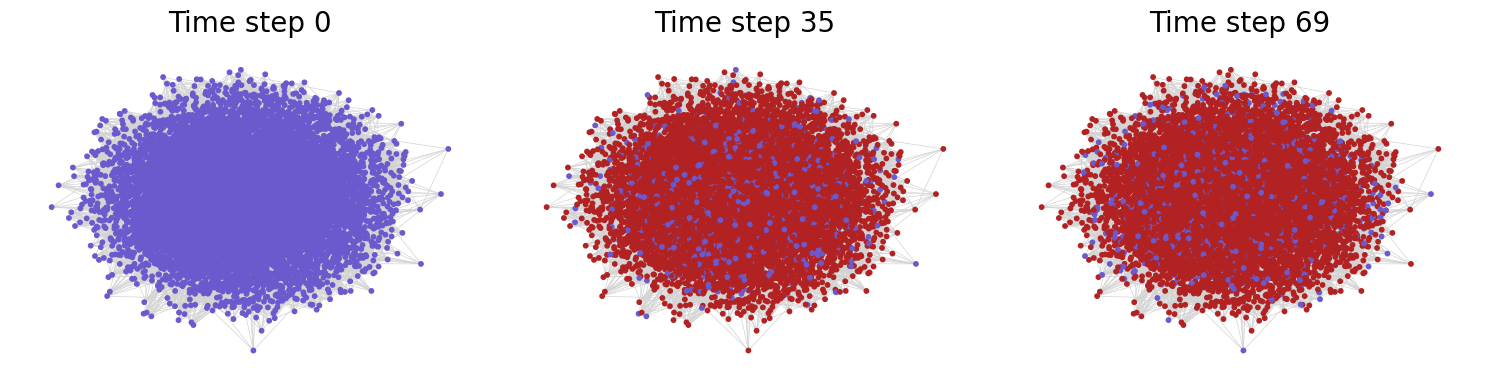
\includegraphics[width=0.8\textwidth]{images/Homogeneous/SIS_snapshots.png}
\caption{Snapshots at $t=0$, $t=T/2$, and $t=T$ for the SIS model.}
\label{fig:sis_snapshots}
\end{figure}

\subsubsection{Mean-Field Equations}
\label{app:full_counts}
Letting $s=S/N$ and $i=I/N$ denote the fractions of susceptible and infected individuals in a population of size $N$, the corresponding mean-field equations for the fractions $s(t)$ and $i(t)$ are:
$$\dfrac{ds}{dt}=-\beta \langle k \rangle si + \mu_S i$$
$$\dfrac{di}{dt}=\beta \langle k \rangle si - \mu_S i$$

We define a binary state variable $\sigma_i(t)$ for each node and the infection probability $\rho(i,t) = \text{Prob}[\sigma_i(t) = 1]$. Assuming spatial homogeneity $\rho(i,t) = \rho(t)$ and statistical independence:
\begin{equation}
\text{Prob}[\sigma_i = 0, \sigma_j = 1] \approx (1 - \rho)\rho.
\end{equation}

The corresponding mean-field equation for the infection probability becomes:
\begin{equation}
\frac{d\rho}{dt} = -\mu \rho + \beta \sum_j A_{ij} (1 - \rho) \rho.
\end{equation}
In homogeneous networks, where each node has the same average degree $\langle k \rangle$, we approximate $\sum_j A_{ij} \approx \langle k \rangle$, yielding:
\begin{equation}
\frac{d\rho}{dt} = -\mu \rho + \beta \langle k \rangle (1 - \rho)\rho.
\label{eq:SIS_hmf}
\end{equation}

This is a logistic-type equation that admits a steady-state solution. If $\beta > \mu / \langle k \rangle$, the infection persists in an endemic state.

The analytical solution of Eq.~\eqref{eq:SIS_hmf}, assuming an initial condition $\rho(0) = \rho_0$, is:
\begin{equation}
\rho(t) = \rho_0 \frac{(\beta \langle k \rangle - \mu) e^{(\beta \langle k \rangle - \mu)t}}{\beta \langle k \rangle - \mu + \beta \langle k \rangle \rho_0 e^{(\beta \langle k \rangle - \mu)t}}.
\label{eq:SIS_analytical_full}
\end{equation}
This solution describes initial exponential growth followed by saturation at a steady-state value $\rho_\infty = 1 - \frac{\mu}{\beta \langle k \rangle}$.

In the early phase of the outbreak, when $\rho \ll 1$, we can approximate:
\begin{equation}
\rho(t) \approx \rho_0 e^{(\beta \langle k \rangle - \mu)t}.
\label{eq:SIS_exp_growth}
\end{equation}

At steady state, setting $d\rho/dt = 0$ in Eq.~\eqref{eq:SIS_hmf} leads to the threshold condition for sustained transmission:
\[
\beta > \frac{\mu}{\langle k \rangle}.
\]
This defines the basic reproduction number $R_0 = \beta \langle k \rangle / \mu$. The epidemic becomes endemic only if $R_0 > 1$. In our network, this gives a threshold value $\beta_c = 0.005$.



\subsection{SI Model}
The simulation results and ODE solution are compared in Figure~\ref{fig:si_compare}.

\subsubsection{Mean-Field Equation}

The mean-field dynamics are governed by the following system of ordinary differential equations:
$$\dfrac{ds}{dt}=-\beta \langle k \rangle si$$ $$\dfrac{di}{dt}=\beta \langle k \rangle si$$
With $\langle k \rangle$ average degree of the network.

In the SI model, there is no recovery, so the probability of being infected can only increase:
\begin{equation}
\frac{d\rho}{dt} = \beta \langle k \rangle (1 - \rho) \rho.
\label{eq:SI_hmf}
\end{equation}

The analytical solution of the mean-field equation~\eqref{eq:SI_hmf}, assuming an initial condition $\rho(0) = \rho_0$, is:
\begin{equation}
\rho(t) = \frac{\rho_0 e^{\beta \langle k \rangle t}}{1 - \rho_0 + \rho_0 e^{\beta \langle k \rangle t}}.
\label{eq:SI_analytical}
\end{equation}
This is a logistic function describing initial exponential growth with rate $\beta \langle k \rangle$, eventually saturating at $\rho = 1$, corresponding to full infection of the population.




\begin{figure}[H]
\centering
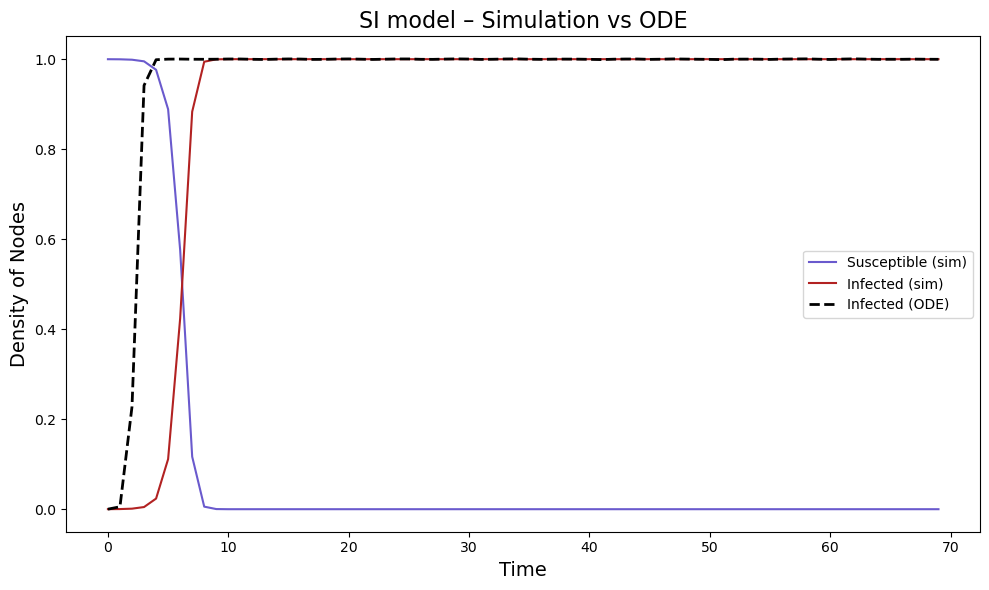
\includegraphics[width=0.6\textwidth]{images/Homogeneous/SI_densities.png}
\caption{Simulation vs ODE integration for the SI model.}
\label{fig:si_compare}
\end{figure}


\subsection{SIR Model}
The simulation results and ODE solution are compared in Figure~\ref{fig:sir_compare}.

\subsubsection{Mean-Field Equations}

The corresponding mean-field equations for the fractions $s(t)$, $i(t)$ and $r(t)$ are:
$$\dfrac{ds}{dt}=-\beta \langle k \rangle si$$ 
$$\dfrac{di}{dt}=\beta \langle k \rangle si - \mu_R i$$
$$\dfrac{dr}{dt}=\mu_R i$$
The SIR model exhibits a stochastic regime in which the infection may die out due to random fluctuations, especially in the early stages.

Although the full model does not admit a closed-form analytical solution, qualitative insights can still be obtained by analyzing its asymptotic behavior as $t=\infty$. 
At $t=\infty$, we have that $i(\infty)=0$ and thus $s(\infty)=1-r(\infty)$, hence the final state is fully characterized by the susceptible and recovered fractions.
$$1-r(\infty)-s_0e^{-r(\infty)\frac{\beta}{\mu_R}}=0$$
This is a trascendental equation that cannot be solved analytically but it gives important hints on the behavior of the disease 
\begin{itemize}
    \item $\dfrac{\beta \langle k \rangle}{\mu_R}=R_0$, determines whether the disease can grow and spread.
    \item $s_0$ plays a central role in shaping the outbreak's outcome. If this fraction is sufficiently low, the infection cannot propagate effectively.
\end{itemize}


\begin{figure}[H]
\centering
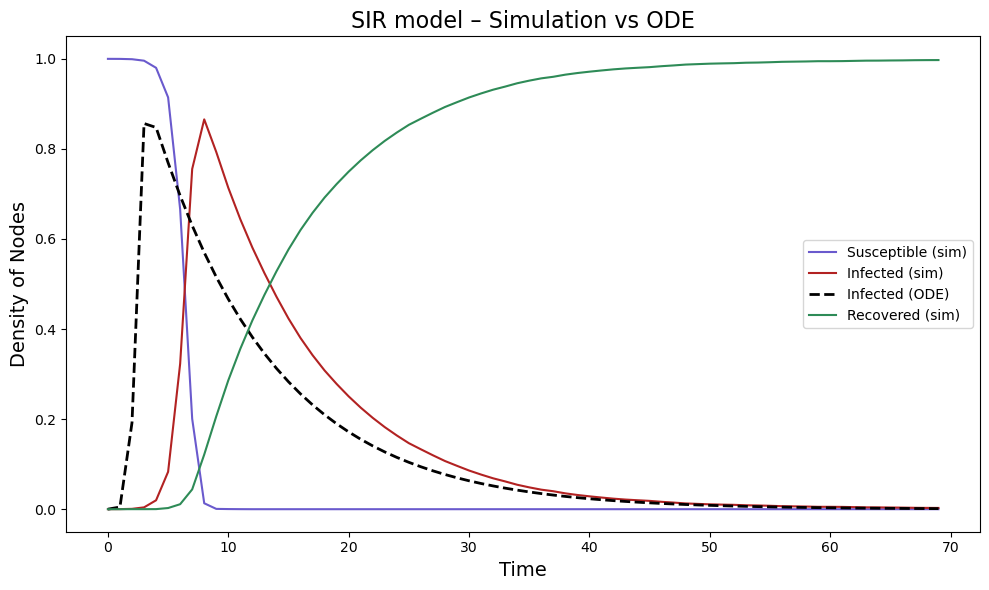
\includegraphics[width=0.6\textwidth]{images/Homogeneous/SIR_densities.png}
\caption{Simulation vs ODE integration for the SIR model.}
\label{fig:sir_compare}
\end{figure}

\subsection{SEIR Model}

\begin{figure}[H]
\centering
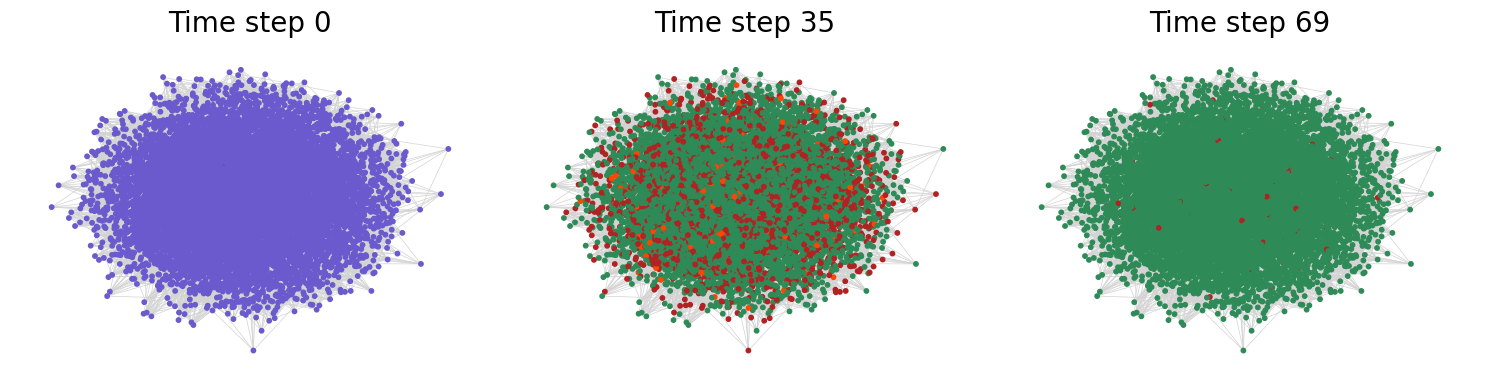
\includegraphics[width=0.8\textwidth]{images/Homogeneous/SEIR_snapshots.png}
\caption{Snapshots at $t=0$, $t=T/2$, and $t=T$ for the SEIR model.}
\label{fig:seir_snapshots}
\end{figure}

\subsubsection{Mean-Field Equations}

The corresponding mean-field equations for the fractions $s(t)$, $i(t)$, $e(t)$ and $r(t)$ are:
$$\dfrac{ds}{dt}= -\beta \langle k \rangle si$$
$$\dfrac{de}{dt}=\beta  \langle k \rangle si - \alpha e$$
$$\dfrac{di}{dt}=\alpha e - \mu i$$ 
$$\dfrac{dr}{dt}=\mu i$$
For very short latent periods—corresponding to the limit $\alpha \rightarrow \infty$, where $\alpha$ is the rate of progression from exposed to infectious—the SEIR model reduces to the classical SIR model, recovering its endemic behavior.

While the steady-state properties—such as the basic reproduction number $R_0$ and the final epidemic size—are often similar between SEIR and SIR models, the inclusion of an exposed compartment introduces a delay in the dynamics. This delay leads to a noticeably slower initial growth of the infection, approximately proportional to the square root of time, compared to the exponential growth seen in the SIR model:
\begin{equation}
\rho_{\text{SEIR}}(t) \approx \rho_0 e^{\left(\sqrt{4(R_0 - 1)\alpha \mu + (\alpha + \mu)^2} - (\alpha + \mu)\right)t/2} \approx \rho_0 e^{(\sqrt{R_0} - 1)\mu t},
\end{equation}
\begin{equation}
\rho_{\text{SIR}}(t) \approx \rho_0 e^{(R_0 - 1)\mu t}.
\end{equation}
Although this difference vanishes at equilibrium, it has substantial implications during the early stages of an outbreak. Accurately capturing such temporal dynamics is crucial for effective early interventions and informed public health decisions.



\begin{figure}[H]
\centering
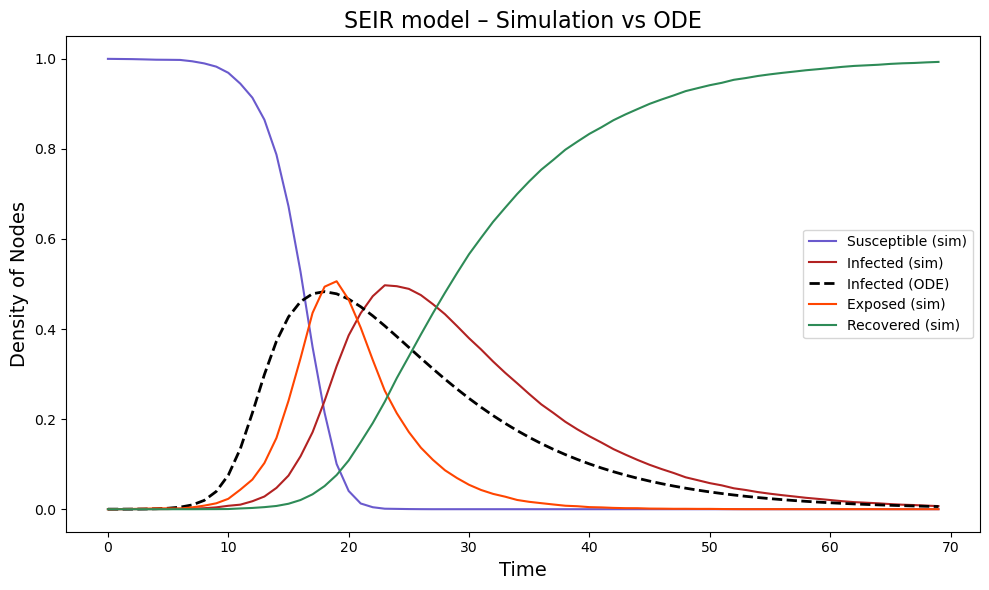
\includegraphics[width=0.6\textwidth]{images/Homogeneous/SEIR_densities.png}
\caption{Simulation vs ODE integration for the SEIR model.}
\label{fig:seir_compare}
\end{figure}

\medskip

\section{Heterogeneous Mean Field Approximation}

\label{app:Heterogeneous_MF}

\subsection{Finite size effects on the SIS critical threshold}
Real-world networks are inherently finite, making it essential to account for finite-size corrections when evaluating epidemic thresholds. A common approach is to introduce an exponential cutoff in the degree distribution: $$P(k) \simeq
k^{-\gamma}e^{-\frac{k}{k_c}}$$
where $k_c$ is a characteristic cutoff degree.
For large $k_c$ and degree exponent $2< \gamma < 3$ the critical infection rate acquires a finite-size correction and is approximated by:
$$\beta_c \simeq \left(\frac{\mu k_c}{k_{min}}\right)^{\gamma-3}$$

\subsection{SIR}

In this appendix, I perform the heterogeneous mean-field analysis for the SIR model, following the methodology presented in the main text.  
We define the densities of susceptible, infected, and recovered nodes of degree \(k\) at time \(t\) as \(\rho_k^S(t)\), \(\rho_k^I(t)\), and \(\rho_k^R(t)\), respectively, with the final recovered density given by  
\[
\rho_\infty^R = \lim_{t \to \infty} \sum_k P(k) \rho_k^R(t).
\]  
The evolution equations for the infected and recovered densities read  
\[
\frac{d\rho_k^I(t)}{dt} = -\mu \rho_k^I(t) + \beta k \rho_k^S(t) \Gamma_k(t),
\]
\[
\frac{d\rho_k^R(t)}{dt} = \mu \rho_k^I(t),
\]
where the susceptible density satisfies \(\rho_k^S(t) = 1 - \rho_k^I(t) - \rho_k^R(t)\).  

Here,  
\[
\Gamma_k(t) = \sum_{k'} \frac{k' - 1}{k'} P(k'|k) \rho_{k'}^I(t),
\]  
represents the probability that a neighbor of a node with degree \(k\) is infected.  

This formalism modifies the epidemic threshold, which becomes  
\[
\beta_c = \frac{\mu \langle k \rangle}{\langle k^2 \rangle - \langle k \rangle}.
\]  

Importantly, for finite networks, the thresholds for the SIS and SIR models differ, i.e.,  
\[
\beta_c^{\text{SIS}} \neq \beta_c^{\text{SIR}}.
\]

\subsection{SI}
In the absence of recovery, the SI model admits a degree-based mean-field description with:
\[
\frac{d\rho_k(t)}{dt} = \beta k \left[1 - \rho_k(t)\right] \Theta(t),
\qquad
\Theta(t) = \sum_{k'} \frac{k' P(k')}{\langle k \rangle} \rho_{k'}(t).
\]
Since no recovery occurs, the infection always spreads throughout the network and there is no epidemic threshold (\(\beta_c = 0\)).

\subsection{SEIR} 
The SEIR model incorporates an exposed compartment with a finite rate of progression to infection. The degree-based equations read:
\[
\begin{aligned}
\frac{d\rho_k^S}{dt} &= -\beta k \rho_k^S(t) \Theta(t), \\
\frac{d\rho_k^E}{dt} &= \beta k \rho_k^S(t) \Theta(t) - \alpha \rho_k^E(t), \\
\frac{d\rho_k^I}{dt} &= \alpha \rho_k^E(t) - \mu \rho_k^I(t), \\
\frac{d\rho_k^R}{dt} &= \mu \rho_k^I(t),
\end{aligned}
\qquad
\Theta(t) = \sum_{k'} \frac{k' P(k')}{\langle k \rangle} \rho_{k'}^I(t).
\]

To compute the epidemic threshold, we linearize the system near the disease-free state. Assuming \(\rho_k^E, \rho_k^I \ll 1\) and \(\rho_k^S \approx 1\), the growth of \(\rho_k^I\) becomes:
\[
\frac{d\rho_k^I}{dt} \approx \alpha \rho_k^E - \mu \rho_k^I, \quad
\frac{d\rho_k^E}{dt} \approx \beta k \Theta - \alpha \rho_k^E.
\]
Solving this linear system yields exponential growth when:
\[
\frac{\beta \alpha \langle k^2 \rangle}{\mu (\alpha + \mu) \langle k \rangle} > 1,
\]
leading to the epidemic threshold:
\[
\beta_c = \frac{\mu (\alpha + \mu) \langle k \rangle}{\alpha \langle k^2 \rangle}.
\]
As in the SIR and SIS cases, \(\beta_c \to 0\) for scale-free networks with \(2 < \gamma < 3\) in the limit \(N \to \infty\), indicating the absence of a threshold in the thermodynamic limit.

\subsection{Threshold Evaluation}
\label{app:Thresholds}
\subsection*{Network structure}

The simulations were performed on a Barabási–Albert (BA) network, a well-known model for generating scale-free networks characterized by a power-law degree distribution. The network was constructed with \( N = 10^4 \) nodes, where each new node is connected to \( m = 4 \) existing nodes during the network growth process. This generates a heterogeneous topology with a heavy-tailed degree distribution, which strongly influences epidemic dynamics and lowers the epidemic threshold compared to homogeneous networks.

The BA model captures the presence of highly connected hubs, which can significantly accelerate the spread of infections and contribute to the vanishing of the epidemic threshold in the thermodynamic limit.

\subsubsection{SIS}
\begin{figure}[H]
    \centering
    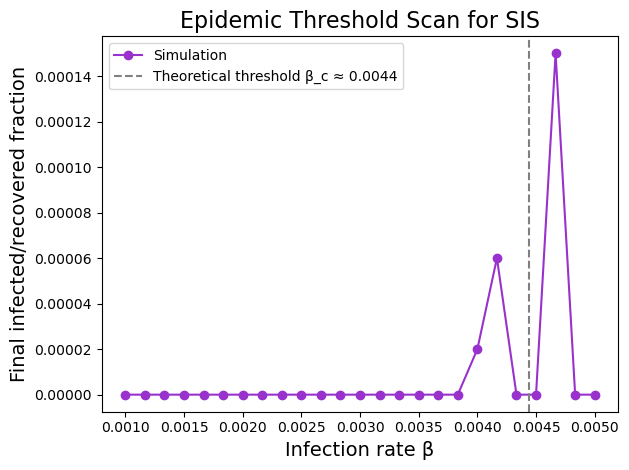
\includegraphics[width=0.5\textwidth]{images/Heterogeneous/SIS_thresholds.png}
    \caption{Epidemic threshold estimation for the SIS model on a heterogeneous network. Each point represents the average infected fraction over multiple runs at fixed infection rate $\beta$.}
    \label{fig:SIS_threshold_heterogeneous}
\end{figure}

The theoretical epidemic threshold in the heterogeneous mean-field approximation is given by:
\begin{equation}
\beta_c = \frac{\mu \langle k \rangle}{\langle k^2 \rangle},
\end{equation}
For the network under study, this gives $\beta_c \approx 0.0044$. However, in simulations, the estimated threshold appears slightly smaller. This discrepancy is due to stochastic effects, finite-size fluctuations, and the fact that the true threshold is better captured by the quenched mean-field theory:
\begin{equation}
\beta_c^{\text{QMF}} = \frac{\mu}{\Lambda_{\max}},
\end{equation}
where $\Lambda_{\max}$ is the largest eigenvalue of the adjacency matrix. In scale-free networks, $\Lambda_{\max}$ can be larger than the mean-field estimate suggests, slightly lowering the empirical critical point observed in simulations.



\subsubsection{SIR}

In this case, I simulate the SIR model on the same Barabási–Albert network described previously. 
\begin{figure}[h!]
    \centering
    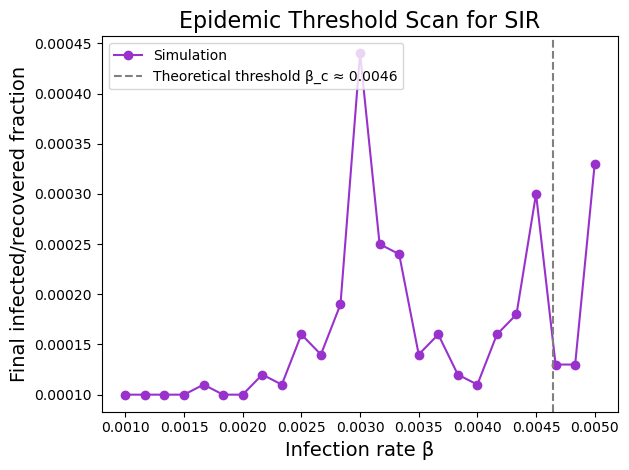
\includegraphics[width=0.5\textwidth]{images/Heterogeneous/SIR_thresholds.png}
    \caption{Epidemic threshold estimation for the SIS model on a heterogeneous network. Each point represents the average infected fraction over multiple runs at fixed infection rate $\beta$.}
    \label{fig:SIS_threshold_heterogeneous}
\end{figure}
The theoretical epidemic threshold in the heterogeneous mean-field approximation is given by:
\[
\beta_c = \frac{\mu \langle k \rangle}{\langle k^2 \rangle - \langle k \rangle}
\]
For the network under study, this gives $\beta_c \approx 0.0046$. 
This threshold indicates the critical point above which a macroscopic fraction of the population becomes infected and then recovers. Once again, we see the discrepancy from the theoretical threshold.

\section{Epidemic spreading on patchy metapopulations: SI, SIS, SIR, SEIR in homogeneous mean-field approximation}
\label{app:Metapopulations}

\subsection*{Invasion Threshold in the SI Model}

The SI model assumes that once infected, individuals remain infectious forever. As a result, there is no recovery and thus no local epidemic threshold; local outbreaks always grow once seeded. The only condition for the epidemic to invade the metapopulation is that infected individuals successfully travel and seed neighboring patches.

In this case, the global invasion depends solely on mobility and the network structure, as there is no saturation or recovery. Every infected individual has infinite infectious duration, so the cumulative probability of infecting neighboring patches approaches one. The focus is therefore on ensuring that the infection reaches a critical number of patches for widespread invasion.


\subsection*{Invasion Threshold in the SIS Model}

In the SIS model, individuals can recover and return to the susceptible state. An infected individual remains infectious for an average time \( \mu^{-1} \), and if \( R_0 > 1 \), the infection reaches an endemic steady state within each patch.

As with the SIR model, a global invasion threshold can be defined using a tree-like approximation. However, the quantity \( \alpha \) is no longer the final size of the outbreak but rather the stationary fraction of infected individuals within a patch.

The global reproductive number for SIS is given by:
\[
R^* = p\bar{N}\alpha\mu^{-1}\frac{\bar{k}-1}{\bar{k}}(R_0 - 1),
\]
and global invasion occurs when \( R^* > 1 \).

\subsection*{Invasion Threshold in the SEIR Model}

The SEIR model introduces a latent (exposed) compartment \( E \), capturing the delay between infection and the onset of infectiousness. The disease progression is \( S \to E \to I \to R \), where exposed individuals become infectious at rate \( \epsilon \), and infectious individuals recover at rate \( \mu \). The change of notation from $\alpha$ to $\epsilon$ for the infection rate is needed because in this notation $\alpha$ is used as the rate of individuals that become infectious during the outbreak.

This latency reduces the effective transmissibility and thus raises the critical threshold. The theoretical threshold in the homogeneous mean-field approximation becomes:
\[
\beta_c = \mu(\mu + \epsilon) \frac{\langle k \rangle}{\epsilon \langle k^2 \rangle}.
\]

Global invasion in the metapopulation is still governed by a condition of the form \( R^* > 1 \), but now the term \( \alpha \) accounts for both delayed infectiousness and the final size of the outbreak, typically lower than in SIR.



\label{app:metapopulations}
\section{Use of ChatGPT}

In this project, ChatGPT \cite{OpenAI2025} primarily assisted in the final revision of the review, refining my initial draft to enhance clarity, professionalism, and appropriateness of language.
It also helped in the coding part, suggesting the best structure to tackle the epidemic simulations, and in finding the papers related to the homogeneous and heterogeneous mean field approximations.

\section{Further acknowledgments}
For the sake of correctness, I acknowledge that part of the material and derivations presented in this review are based on the lecture slides from the course on epidemic modeling taught by Prof. Sandro Meloni.
